\documentclass[a4paper,utf8]{article}
\usepackage{graphicx}
\usepackage[heading,fancyhdr]{ctex}
\usepackage{amsmath,amssymb,geometry,ulem}
\usepackage{array,tabularx,tabulary,mhchem,xspace}
\usepackage{floatrow,subfig,multirow,bigstrut}
\usepackage{siunitx,booktabs,longtable,nameref}
\lineskiplimit=1pt
\lineskip=3pt
\geometry{
    top=25.4mm, 
    left=25mm, 
    right=25mm, 
    bottom=25mm,
    headsep=5.9mm,
}
\ctexset{
    chapter = {
        name = {实验,},
        beforeskip = {-23pt}
    }
}
\newcommand{\fgref}[1]{图~\ref{#1}\xspace}
\newcommand{\seqref}[1]{式~(\ref{#1})}
\newcommand{\expinfo}[6][无]{
    {\zihao{-3}\bfseries\songti
    实验名称:\uline{\hfill\mbox{#2}\hfill} \\[2.9mm]
    学\quad 号:\uline{\makebox[25mm]{#3}}\hfill
    姓\quad 名:\uline{\makebox[25mm]{#4}}\hfill
    班\quad 级:\uline{\makebox[25mm]{#5}} \\[2.9mm]
    合作者:\uline{\makebox[25mm]{#1}} \hfill
    桌\quad 号:\uline{\makebox[25mm]{}}\hfill\makebox[25mm+4em]{}\\[2.9mm]
    指导教师:\uline{\makebox[30mm]{#6}}\hfill\mbox{} \\[2.9mm]
    实验日期:\uline{\makebox[30mm]{}}\hfill\mbox{} \\[58.7mm]
    }
}%\expinfo[合作者]{实验名称}{学号}{姓名}{班级}{指导教师}
\newcommand{\pointingbox}{
    {\zihao{4}\bfseries\songti%
    实验考核\\[3mm]
    \extrarowheight=3mm
    \begin{tabularx}{150mm}{|X|X|X|X|X|}\hline
        \hfil 项目 \hfil  & \hfil 实验预习 \hfil & \hfil 实验过程 \hfil & \hfil 分析与讨论 \hfil & \hfil 总评 \hfil \\[3mm] \hline
        \hfil 评价 \hfil &  &  &  &  \\[3mm] \hline
    \end{tabularx}
    }
}
\newcommand{\derivative}[2]{\frac{\mathrm{d} #1}{\mathrm{d} #2}}
\newcommand{\thinking}[2]{\textbf{#1}\\
答:\begin{minipage}[t]{0.85\textwidth}
    #2
\end{minipage}}

\pagestyle{fancy}
\fancyhf{}
%\fancyhead[C]{材料科学基础实验}
%\fancyfoot[C]{\thepage}
\fancyhead[EC]{\leftmark} \fancyhead[OC]{\rightmark}
\fancyhead[EL,OR]{\thepage}
\fancypagestyle{plain}{\renewcommand{\headrulewidth}{0pt}\fancyhf{}}

\newcounter{Rownumber}
\newcommand*{\Rown}{\stepcounter{Rownumber}\theRownumber}
\newcounter{sample}
\newcommand*{\Sam}{\stepcounter{sample}\thesample}
\newcounter{Fignumber}
\newcommand*{\Fign}{\stepcounter{Fignumber}\theFignumber}

\newcommand*{\resetRown}{\setcounter{Rownumber}{0}}
\newcommand{\qrange}[3]{\qtyrange[range-phrase = \text{$\sim$},range-units =single]{#1}{#2}{#3}}
\floatsetup[table]{capposition=top}
\newcolumntype{C}{>{\hfil}X<{\hfil}}
\renewcommand{\Nameref}[1]{\textbf{\ref{#1}~\nameref{#1}}}
\newcommand{\TTR}[0]{\watt\per\m\per\K}
\usepackage{graphicx}
\graphicspath{{img/}}
\begin{document}
\begin{center}
    {\mbox{}\\[7em]\zihao{2}\bfseries\songti%
    材料科学基础实验报告}\\[34mm]
    \expinfo{Sn-Bi 合金相图的测定}{22301056}{王俊杰}{22 材物}{艾斌}
    {\zihao{4}\bfseries\songti
    实验考核\\[3mm]
    \extrarowheight=3mm
    \begin{tabularx}{150mm}{|X|X|X|X|X|}\hline
        \hfil 项目 \hfil  & \hfil 实验预习 \hfil & \hfil 实验过程 \hfil & \hfil 分析与讨论 \hfil & \hfil 总评 \hfil \\[3mm] \hline
        \hfil 评价 \hfil &  &  &  &  \\[3mm] \hline
    \end{tabularx}
    }
\end{center}
\newpage
\section{实验目的}
    \begin{itemize}
        \item 学会用热分析法测绘 Sn-Bi 合金相图;
        \item 了解纯金属和二元合金步冷曲线形状的差异;
        \item 学会从步冷曲线上确定相变点温度的方法;
        \item 学会根据实测的步冷曲线绘制相图
    \end{itemize}
\section{实验原理}%简单描述,含必要的公式和附图;
    相图是描述热力学平衡条件下系统中相与温度、成分和压强之间关系的图解,也称为平衡状态图。相图对于指导材料的加工(凝固、热处理)和预测材料的组织结构及性能具有很高的实用价值和参考意义。测量二元合金相图的关键是要准确测定出各成分合金的相变临界点。所谓相变临界点是指物质结构和性质发生本质变化的临界点。目前已发展出多种测定材料相变临界点的方法,譬如热分析法、热膨胀法、电阻测量法、磁特性测量法、显微分析法、X 射线衍射分析法等。这些方法都是利用材料发生相变时伴随着相关物理性能或组织结构发生突变这一特点进行测量的。热分析法是一种简单易行的测量相图的方法。对于由液相转变为固相的相变临界点的测定,热分析法准确可靠,但是对于因降温溶解度超出固溶度极限从固溶体中析出另一固相的情形,因所释放的相变潜热较小而难以用热分析法测定相变临界点。因此,准确测量二元合金的完整相图通常需要多种方法配合使用。本实验使用热分析法测绘 Sn-Bi 合金相图。\par
    首先,按质量分数配制一系列不同组分比例的有代表性的 Sn-Bi 混合物。然后,分别将所配制的 Sn-Bi 混合物、纯 Sn 和纯 Bi 样品加热熔化成单一、均匀的液相,然后让各样品缓慢冷却,并每隔一定时间读取一次各样品的温度,由此可得到各样品的温度随时间变化的曲线,称为冷却曲线或步冷曲线。对于纯 Sn 或纯 Bi,随着温度的降低,液相的温度不断降低,由于不涉及相变,温度下降的速率较均匀。当继续冷却,纯金属的冷却曲线将出现一个温度保持不变的平台期,平台对应的温度为材料的凝固温度。平台期的起点(左边的拐点)表示液相中开始有固相析出。平台期的终点(右边的拐点)表示液相刚好全部凝固为单一固相。中间的平台期对应于固、液两相共存的阶段,由相律公式 $f=C-P+1$ 可知,此时自由度为零,所以温度保持不变,表示纯金属在恒温下凝固。经过平台期的终点之后,随着继续冷却,体系的温度也将继续下降。对于一定组成的 Sn-Bi 混合物,随着温度的降低,液相的温度不断降低。当温度达到相变温度时,固相(Sn-Bi 固溶体)开始从液相中析出,凝固释放相变潜热,使体系降温的速率变慢,步冷曲线的斜率发生变化而出现第一个拐点。随着继续冷却,更多的固相从液相中析出。由相律公式 $f=C-P+1$ 可知,二元合金凝固(液、固两相共存)时体系的自由度为 1,这意味着随着冷却的进行,温度会继续下降。当液相全部凝固为固相时,由于没有新的相变潜热释放,步冷曲线的斜率将再次改变而出现第二个拐点。随着继续冷却,体系的温度也将以另一速率下降。总之,不同于纯金属的步冷曲线,合金的步冷曲线上没有平台,而是存在两次转折,温度较高的转折点对应于凝固开始的温度,而温度较低的转折点对应于凝固结束的温度。由步冷曲线测定的每个相变临界点在以合金成分为 x 轴、温度为 y 轴的二元系相图中都分别对应一个点,将所有意义相同的临界点(凝固的起始点或终止点)连接起来就得到了 Sn-Bi 合金相图。
    
\section{实验仪器}%规格及参数
    JX-3D8 金属相图测量装置,计算机。
\section{实验过程}%简述主要过程和实验内容
    本实验使用的 JX-3D8 金属相图测量装置配备有计算机和“金属相图(8 通道)实验软件”。利用计算机和该软件可以自动采集、实时显示和保存 8 个样品管中试样的步冷曲线。步冷曲线测试结束后,实验人员需要从步冷曲线或步冷曲线数据上寻找和确定相变点(或拐点)温度,然后,在操作软件的“查看”下拉菜单中选择“相图”出现绘制相图界面,在操作界面左侧相应的数字框中填入拐点温度、成分、平台温度、共晶成分和共晶温度,由软件绘制出相图。
\section{实验结果}
\subsection{机器直接绘制的相图}
\begin{figure}[!ht]
    \begin{floatrow}
        \ffigbox[0.4\textwidth]{\caption{全过程温度变化曲线}}{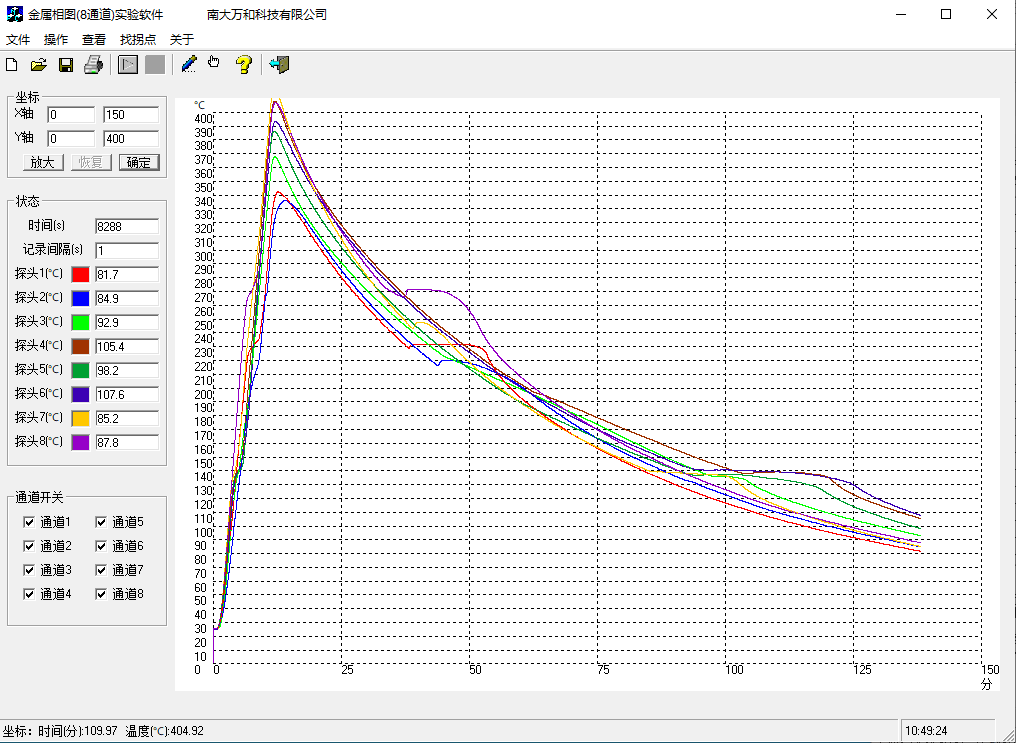
\includegraphics[width=0.4\textwidth]{curve.png}}\hspace{10mm}
        \ffigbox[0.4\textwidth]{\caption{机器绘制相图}}{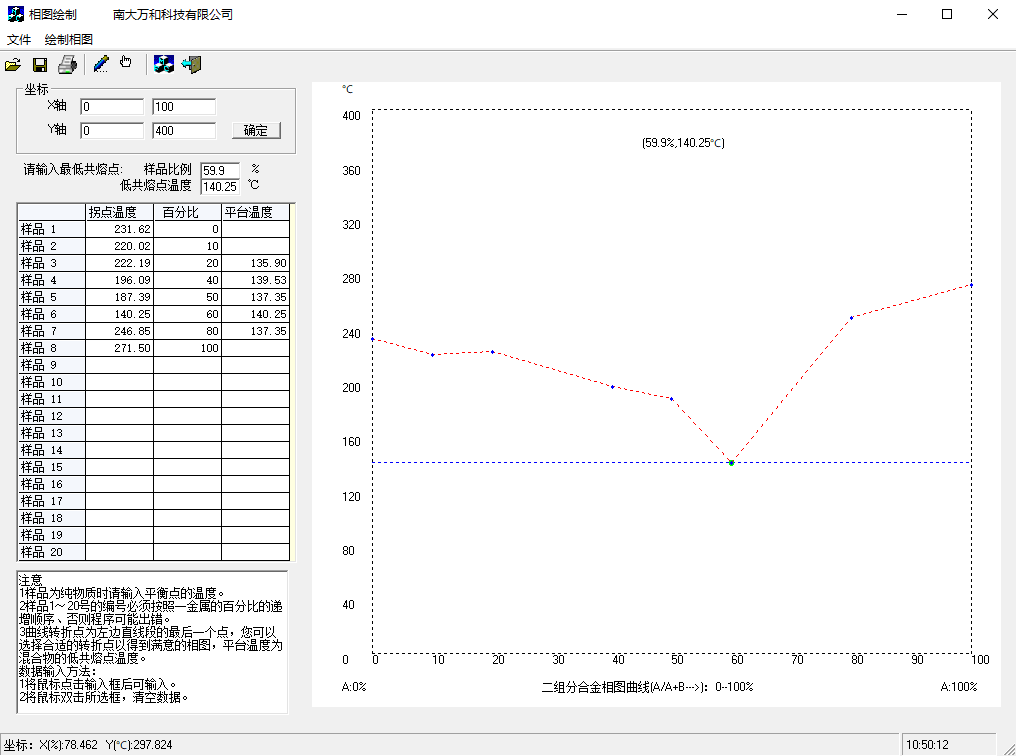
\includegraphics[width=0.4\textwidth]{xiangtu.png}}
    \end{floatrow}
\end{figure}
\subsection{处理后的相图}
\begin{figure}[!ht]
    \caption{Sn-Bi 合金相图}
    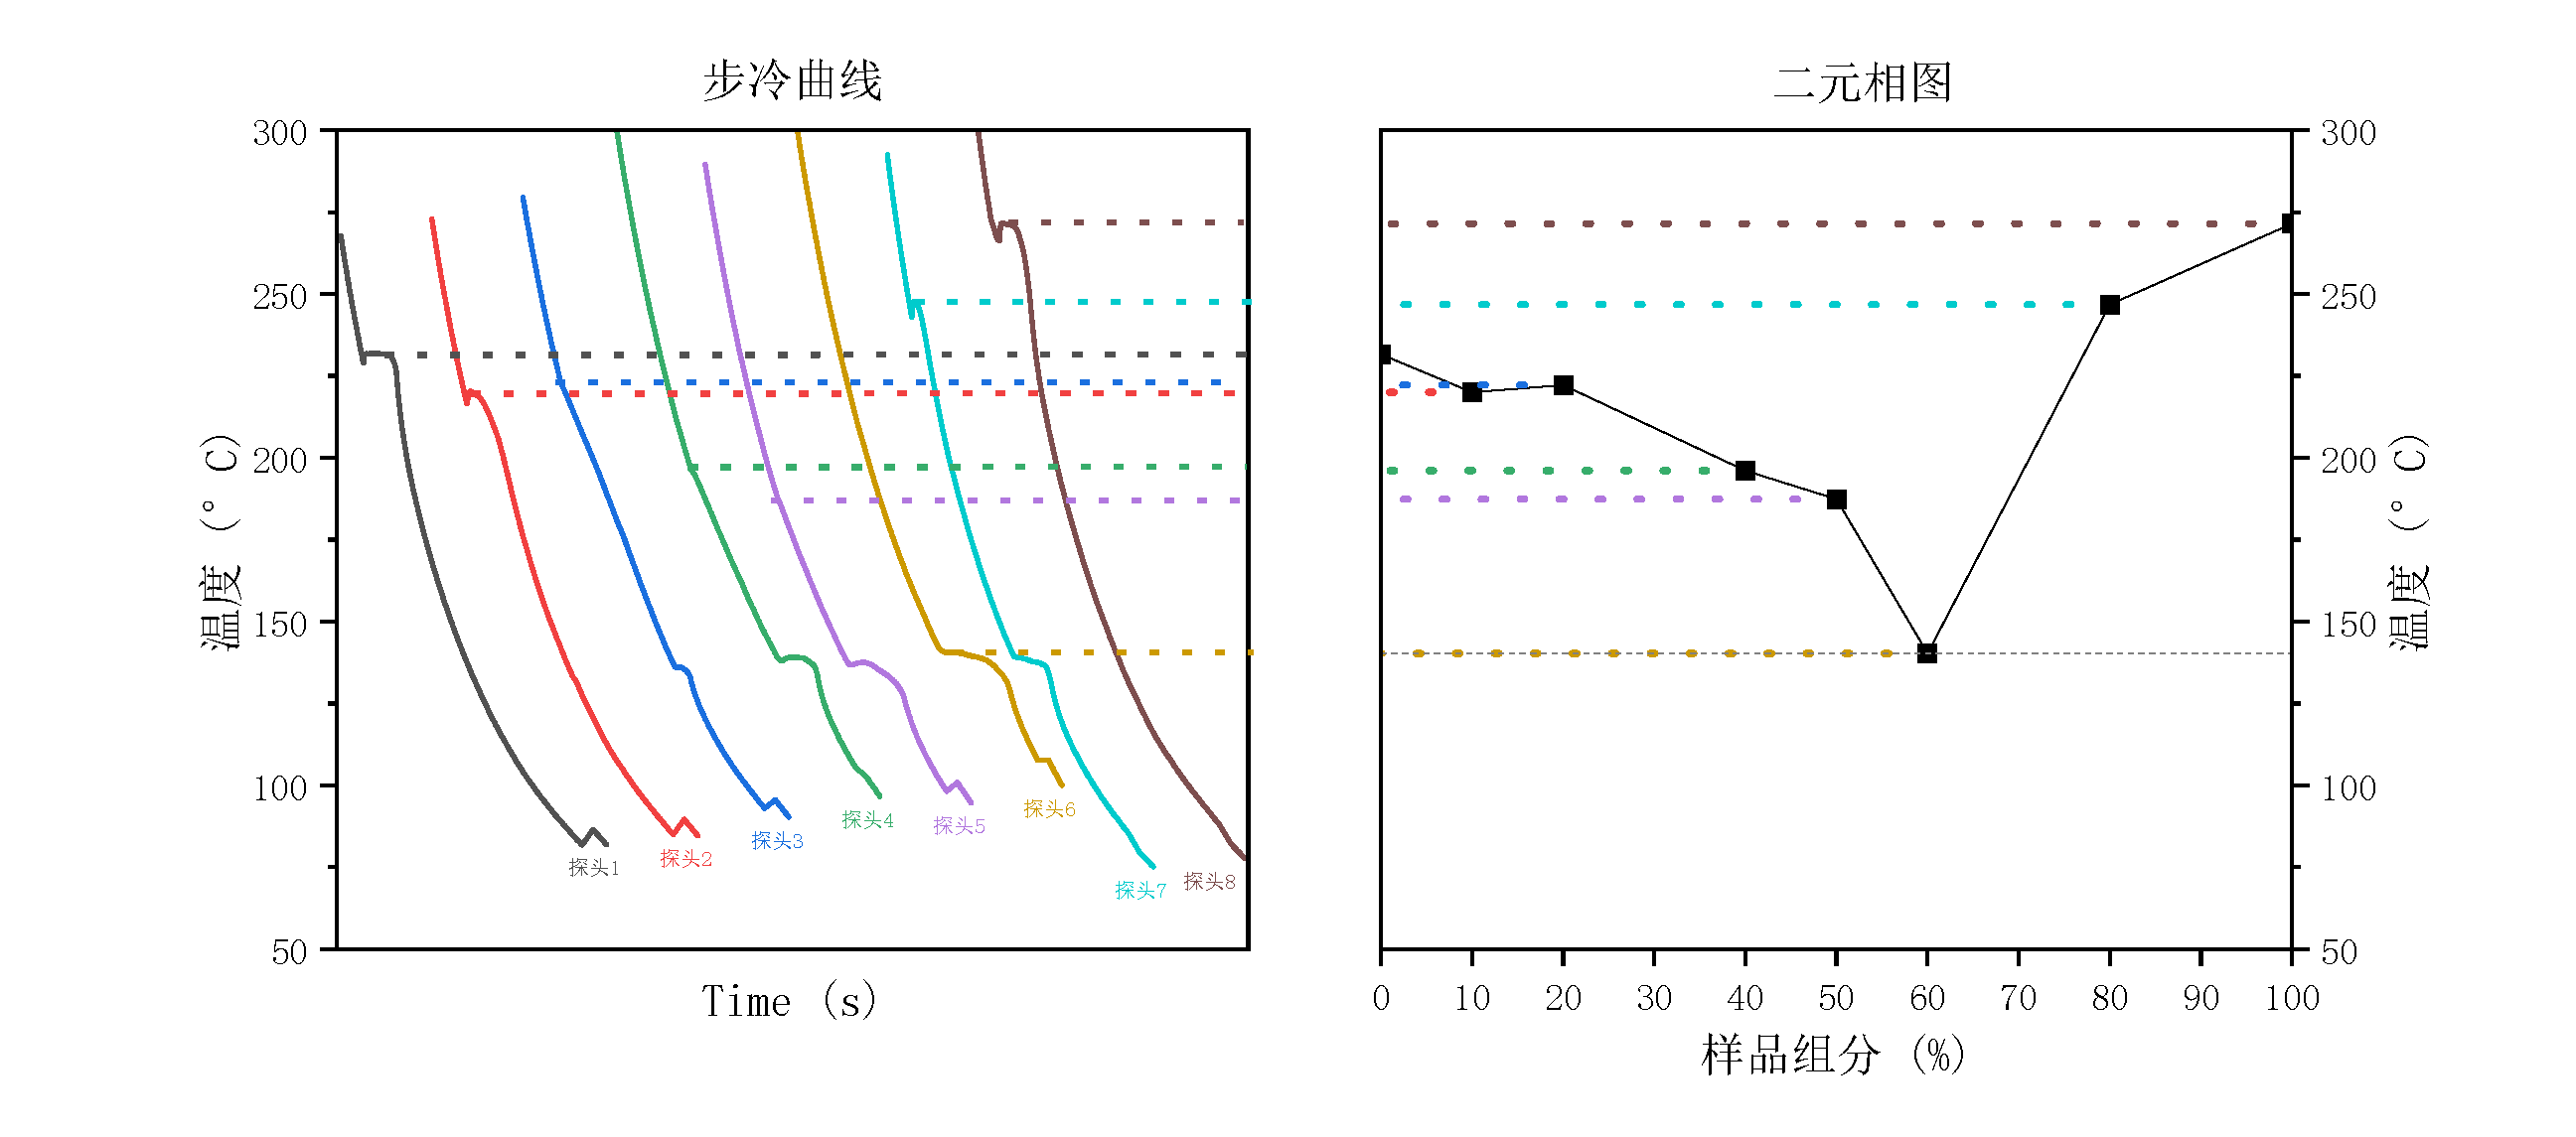
\includegraphics[width=0.9\textwidth]{figwjj.pdf}
\end{figure}

\section{思考题}
\begin{enumerate}
    \item \thinking{要想用热分析法准确测出相图,实验中应注意哪些事项?}{
        \begin{enumerate}
        \item 冷却速度不宜过快,否则转折点将不明显。
        \item 根据相律,降温时条件的改变将会改变自由度、从而出现转折点,所以应当从某一温度起严格保持降温条件一致,以获得准确的相图。
        \end{enumerate}
    }
    \item \thinking{纯金属和二元合金步冷曲线形状有何不同?试利用相律的知识进行解释。}{对于纯金属,步冷曲线呈现出以下特点:随着温度的降低,液相的温度也会持续下降,因为纯金属不涉及相变,所以温度下降的速率比较均匀。在继续冷却后,纯金属的冷却曲线将出现一个温度保持不变的平台期,平台对应的温度为材料的凝固温度。这是因为在平台期间,固、液两相共存,根据相律公式 $f = C−P +1$,自由度为零,使得温度保持不变,表示纯金属在恒温下凝固。经过平台期后,随着继续冷却,体系的温度将继续下降,表示纯金属进一步凝固。\\
    对于二元合金,步冷曲线的特点如下:随着温度的降低,液相的温度也会下降,但在相变温度时,开始有固相从液相中析出,释放相变潜热,使得体系降温速率变慢,步冷曲线的斜率发生变化,出现第一个拐点。随着继续冷却,更多的固相会从液相中析出,根据相律公式 $f = C − P + 1$,二元合金凝固(液、固两相共存)时体系的自由度为 1,这意味着随着冷却的进行,温度会继续下降。当液相全部凝固为固相时,由于没有新的相变潜热释放,步冷曲线的斜率将再次改变,出现第二个拐点,表示凝固过程的结束。}
    \item \thinking{有一失去标签的 Sn-Bi 合金样品,用什么方法可以确定其组成?}{测定其步冷曲线,根据曲线上有无平台、转折点的位置,对照标准样品的步冷曲线来确定其组分。}
    \item \thinking{仅使用热分析法能测出完整的Sn-Bi合金相图吗?为什么?}{不可以,热分析法得到的离散数据即使拟合也无法得到完整的相图,而要得到完整的相图,应该根据相变吉布斯自由能来计算出理论的相图。}
\end{enumerate}
\end{document}